
\chapter{Introduction and motivation}
The introducing chapter of this thesis is dedicated to impart an overview of vacuum metrology and the current state of the art when it comes to mechanical pressure standards in the vacuum region. With the prospect of photon based alternatives, the project and thesis goals are discussed.
 \section{QuantumPascal project}
The QuantumPascal project is a joint research project of eleven European metrological institutes and one industrial partner (See Fig. \ref{Parnter_institutes}). The idea of the project is to develop new photon-based methods to measure gas pressures precisely and thereby counteract the decade long stagnation in improving the widely used mechanical counterparts like piston gauges or mercury manometers.
\begin{figure}[H]
	\centering
	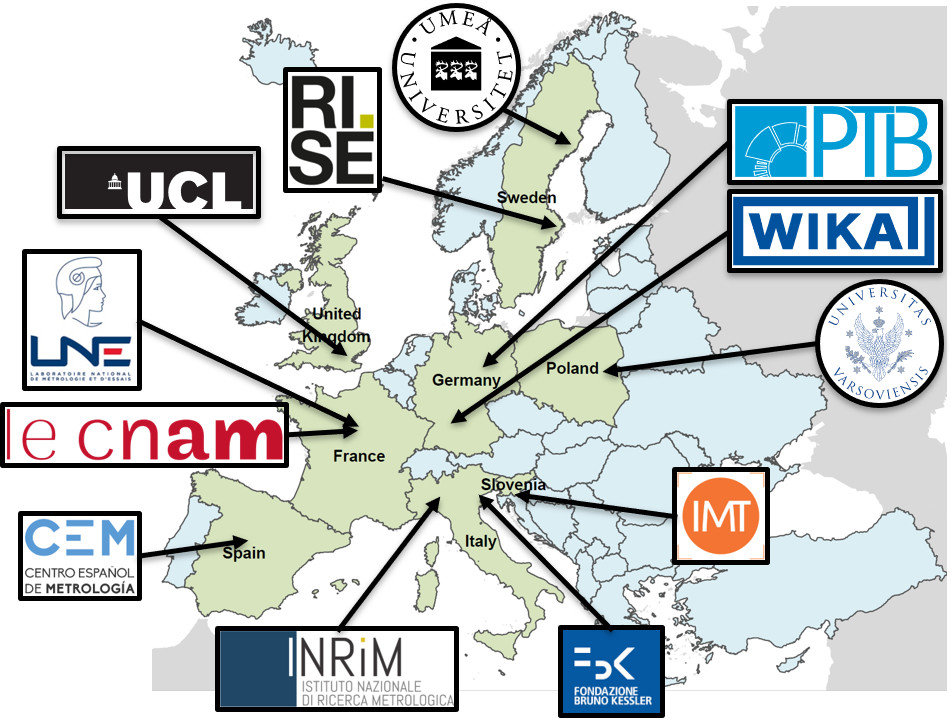
\includegraphics[width=0.7\textwidth]{/Einleitung/Partner_institutes}
	\caption{Shown are all participating institutes, universities and companies of the QuantumPascal project. Each partner focusses either on developing new photonic pressure standards or calculating relevant theoretical gas properties. }
	\label{Parnter_institutes}
\end{figure}
\noindent
 By developing new quantum based pressure standards and calculating the required thermodynamic and electromagnetic gas properties, the project seeks to pave the way towards a quantum-based realisation of the pascal vial the ideal or real gas law. The gas pressure is then accessed with gas density measurements opposed to the classical way of determining the pressure mechanically by measuring the force that acts on a defined area.
 \begin{equation}
 P= \frac{F}{A} \; \xRightarrow[\text{change}]{\text{System}} \; P = \rho k_B T
 \label{System_change}
 \end{equation}
 Many industrial sectors, like the semiconductor industry, greatly benefit from improved gas-pressure measurements within their production routine. The required measurement device calibration is ultimately provided by the respective national metrological institute.  But also other applications, like the scientific backtracing of greenhouse gases, can advance in accuracy and diversity if new and improved gas density measurement systems are created. Switching from mechanical pressure standards to photon based standards is justified by a chain of arguments which evolve around the outstanding potential to improved the overall measurement uncertainties. With the new definition of the SI-system in May 2019 many natural constants, like the Boltzmann constant k$_b$, were assigned an uncertainty of zero. Since most photonic methods measure gas densities that are related to gas pressure via the ideal or real gas law, the new definition of the SI-system also benefits optical gas pressure measurements. The recent advancement in Laser technology also justifies a change from mechanical to optical standards. On one hand the development of quantum cascade lasers in 1994 by J. Faist et al \cite{Faist1994} created a vast amount of Laser sources in the molecular fingerprint region of the EM-spectrum. Thus allowing the construction of partial pressure standards for virtually any gas of the region when absorption spectroscopy is used as a primary measurement technique. On the other hand the frequency of laser light can be stabilized with an uncertainty of up to $\delta \nu$ $=10^{-17}$ \cite{Haefner2015}. But also other relevant optical properties apart from the frequency of light have been theoretically determined with excellent uncertainties. One important example is the refractivity of helium which is known with a relative uncertainty of $10^{-6}$ and therefore makes refractivity measurements an outstanding candidate for new gas pressure standards. 
\section{Pressure standards at the PTB}
The PTB (Physikalisch-Technische-Bundesandtalt) is the national metrology institute of Germany. The working groups 3.33 ("Pressure") and 7.54 ("Vacuum metrology") currently realize the pressure scale from atmospheric pressure up to the ultra high vacuum region with different mechanical pressure standards. Four different methods and their respective relative uncertainties are shown in Fig. \ref{Pressure_standards_status_quo}.\\\\ A \textbf{mercury manometer} is used to determine the pressure difference P$_1$-P$_2$ that is present between the two surfaces of a mercury filled, U-shaped tube. The height difference of the two liquid columns can be measured precisely with interferometric methods and is directly proportional to the applied pressure difference $\Delta $P:
\begin{equation}
\Delta P = \rho \cdot g \cdot h
\label{Hg-manometer}
\end{equation}
with the gravitational constant $g$ and $\rho$ the density of mercury. The manometer can be used for pressure measurements from athmospheric pressure down to 100 Pa. The relative uncertainty of the mercury manometer surpasses most other gauges and goes as low as $10^{-6}$ at atmospheric pressure. The pressure balance is only limited by the density measurement of mercury and the temperature stability of the tube.
\newpage 
\begin{figure}[H]
	\centering
	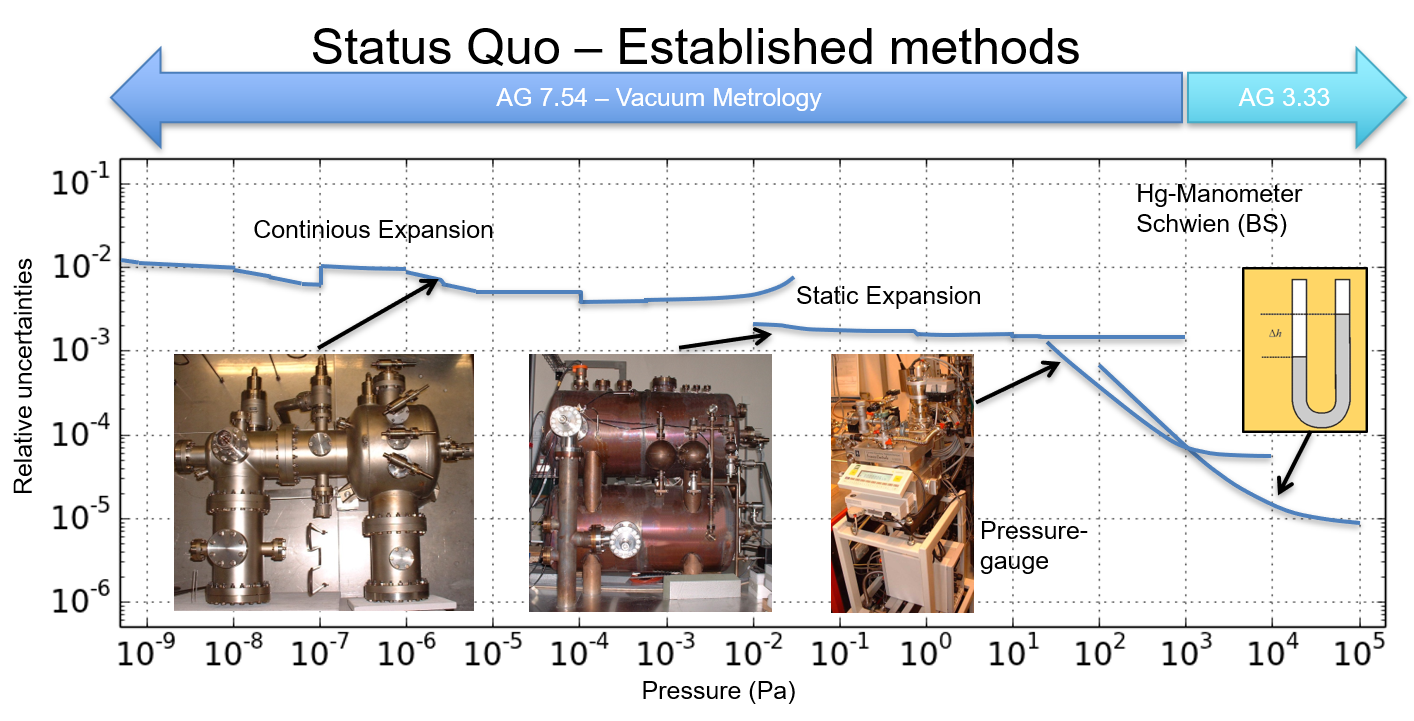
\includegraphics[width=0.9\textwidth]{/Einleitung/Statsus-Quo-Pressure-standards-PTB}
	\caption{Shown are the mechanical pressure standards which are used by the PTB with their respective relative uncertainties, aswell as the vacuum range they cover. Graphic taken from \cite{Rubin2016}.}
	\label{Pressure_standards_status_quo}
\end{figure}
\noindent
A \textbf{pressure gauge} is a primary pressure standard that can generate a gas pressure between 10 Pa and 10 kPa. To generate the pressure, a well known rotating piston is positioned inside a tightly fitted tube. One surface of the piston is directly in contact with the measurement gas while the second cross sectional surface of the piston is en-capsuled in an evacuated glass bell. Once the downwards acting weight force of the piston equals the pressure that the gas asserts on the surface area of the piston, a well defined pressure difference P$_1$-P${_2}$ is created between the two sides of the piston. Since the pressure P$_1$ on the encapsuled side is known, e.g by calibration with a mercury manometer, the piston gauge can be used to calibrate commercially available pressure measurement devices. The relative uncertainties of a piston gauge go as low as 10$^{-5}$ but require precise alignment of the piston since additional frictional or electrical forces have to be avoided.\\\\
\noindent
The \textbf{static expansion} is a primary pressure standard that can generate gas pressures between 10$^{-2}$ Pa and 1 kPa. The combined gas law:
\begin{equation}
\frac{P_1\cdot V_1}{T_1} = \frac{P_2\cdot V_2}{T_2}
\label{Boyle-Mariotte-law}
\end{equation}
is used to determine the target pressure P${_1}$. This target pressure is experimentally generated by expanding a compressed gas at a pressure P$_2$ from a well known small volume V${_2}$ into a large volume V$_1$. The relative uncertainty of the static expansion is in the order of 10$^{-3}$ for most of the covered vacuum region. A limiting factor is often the temperature stability of the system, especially in the expansion chambers.\\\\ The \textbf{continuous expansion} is used in the high and ultra high vacuum region. The generated pressure is scaled down by continuously expanding the measurement gas into a vacuum pump via two precisely defined conductances. The first orifice connects the gas filled expansion chamber (with a pressure P$_1$) with the measurement chamber, in wich the target pressure P$_2$ is going to be generated. The second orifice has a much larger conductance than the first one (C$_2$$\gg$C$_1$) and connects the measurement chamber with the vacuum pump (P$_3$). A continuous flow is created and the pressure significantly decreases after each orifice. Under isothermal conditions the flow through both conductances has to be equal. Since the expansion chamber is under high pressure (P$_1$$\gg$ P$_2$ $\gg$ P$_3$) it follows a simple formula to determine the target pressure P$_2$ in the measurement chamber \cite{Jousten2016}.
\begin{equation}
(P_1-P_2) C_1 =(P_2-P_3)C_2 \xRightarrow[\text{P$_1$$\gg$ P$_2$ $\gg$ P$_3$}]{\text{with}} \; P_2=P_1 \frac{C_1}{C_2}
\label{isothermal-condition}
\end{equation}
By choosing a reasonable combination of orifices, the continuous expansion can generate UHV pressures up to 10$^{-9}$ Pa and achieve relative uncertainties between 10$^{-2}$ and 10$^{-3}$. Limiting factors of the method are the gas dependant leak rate of the very small conductance (C$_1$) as well as temperature stability of the system.\\\\ 
All four methods full fill the requirements of a well designed pressure standard: The pressure can be determined from a simple physical context, allowing high control of potential error sources and thus benefiting repeatability and overall performance.
\section{Development of photon based methods at the PTB}
The newly founded working group 7.55 ("Photonic pressure measurements") is dedicated to developing new pressure standards within the QuantumPascal project. Two independent systems are developed, both with promising prospects regarding the overall measurement uncertainty of pressure measurements. Figure \ref{Pressure_standards_photonic} shows an uncertainty comparison of the existing mechanical pressure standards (in blue) and a selection of photonic pressure standards (in red). The relative uncertainties of the quantum based methods are estimated based on existing setups at other metrology institutes and the green arrows indicate the potential of further decreasing those by improving the respective experimental setup. The absorption spectroscopy setup, as well as the refractometer will be developed and build at the PTB. 
\begin{figure}[H]
	\centering
	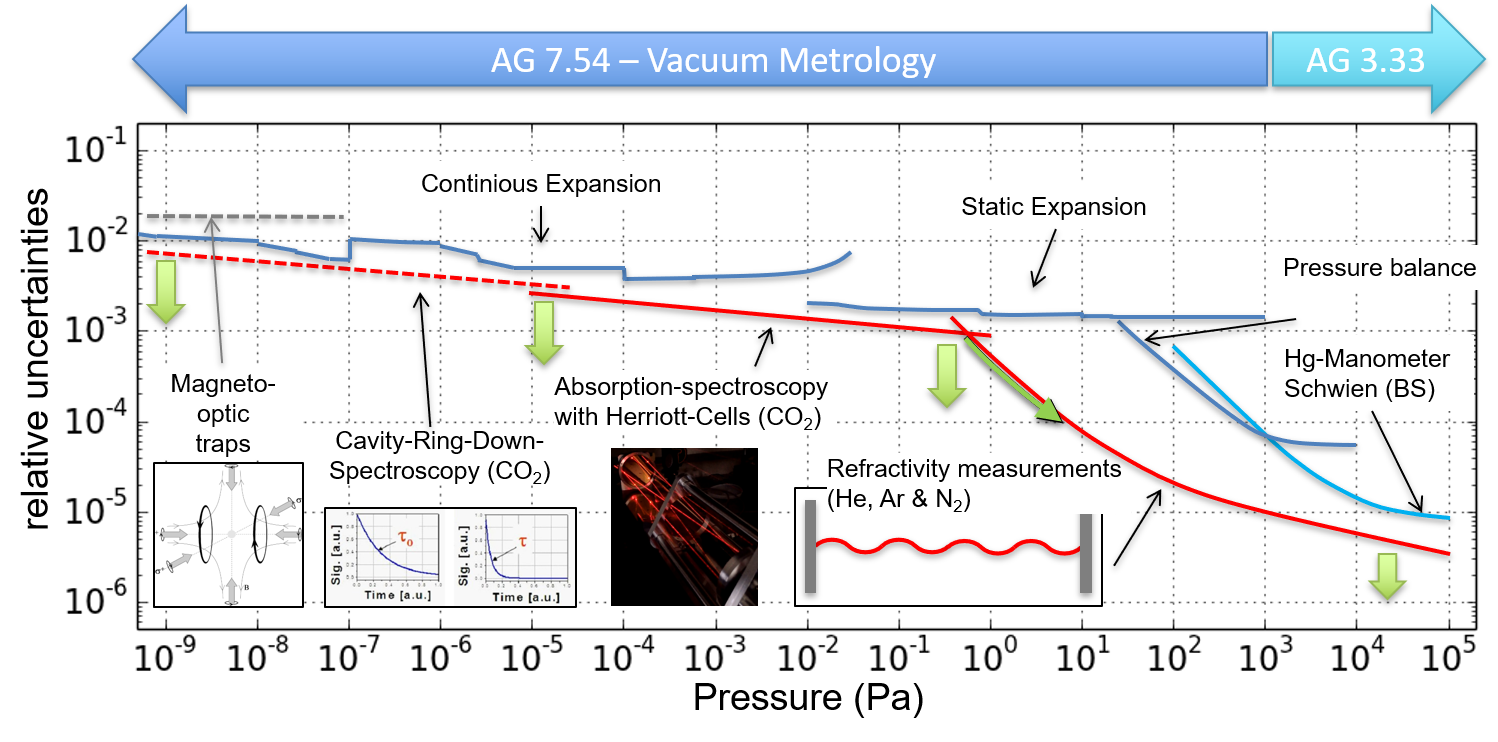
\includegraphics[width=0.9\textwidth]{/Einleitung/Optical-Pressure-standards-PTB}
	\caption{Comparison of the uncertainties of the established mechanical pressure standards at the PTB and the potential uncertainties of the new photonic pressure standards, of which some are being build during the QuantumPascal project by the AG 7.55. Image taken from \cite{Rubin2016}.}
	\label{Pressure_standards_photonic}
\end{figure}
\noindent
A \textbf{refractometer} can be used as a photon based pressure standard. The operating principle relies on the pressure dependent refractive index of gases, which can be measured using lasers. Therefore a Laser with the wavelength $\lambda$ is locked to a gas filled resonator with a length L, so that the standing wave condition is fulfilled:
\begin{equation}
L= \frac{\lambda}{2\cdot n}\cdot \text{integer}
\label{standing-wave-condition}
\end{equation}
The lock depends on the refractive index of the gas and to upkeep the standing wave inside the resonator, the laser wavelength has to be adjusted according to the pressure induced change in the refractivity. The laser frequency change $\Delta$f is proportional to the change in refractivity:
\begin{equation}
\frac{\Delta f}{f} \propto (n-1)
\label{standing-wave-condition}
\end{equation}
This simple correlation can be combined with the Lorentz-Lorenz equation to determine the density of the gas. 
\begin{equation}
\rho= \frac{3\cdot\epsilon_0}{\alpha}\cdot \frac{n^2-1}{n^2+2}
\label{Lorentz-Lorenzn}
\end{equation}
Once the gas density is obtained, the pressure of the gas filled resonator can be calculated using the ideal or real gas law. Potentially problematic are the temperature stability of the system, the gas purity and the length stability of the resonator.\\\\
\noindent
An \textbf{absorption spectroscopy} setup can be combined with an optical multipass cell to form an effective pressure standard. The Lambert Beer law of absorption describes how much light intensity is absorbed by a medium, in this case a gas, after the light travelled through a fixed distance L of that medium. 
 \begin{equation}
 I = I_0 \cdot e^{ -\alpha \rho L } \Leftrightarrow \rho = - \text{Ln}(\frac{I}{I_0})/(\alpha L)
 \label{introduction-lambert-beer}
 \end{equation}
The amount of remaining light intensity depends on the coefficient of absorption $\alpha$ as well as the gas density $\rho$.  Solving for the gas density and combining the Lambert-Beer law with the ideal gas law, makes absorption spectroscopy a promising  new optical pressure standard. The challenges are  to generate reasonably long optical path lengths to enable low gas density measurements in the high vacuum region as well as narrowing the linewidth of the commonly used quantum cascade lasers. This thesis is dedicated to developing, building and improving a fully automatic optical pressure standard at the PTB, by using absorption spectroscopy together with a multipass cell type which was designed by D.R Herriott in 1965.
\newpage